\chapter{Конструкторская часть}

\section{Схема алгоритма нахождения расстояния Левенштейна}

На рисунке \ref{img:recursive} приведена схема рекурсивного алгоритма нахождения расстояния Левенштейна.

На рисунке \ref{img:init_matrix} схема алгоритма инициализации матрицы.

На рисунках \ref{img:rec_mem} и \ref{img:recursive_with_mem} приведена схема рекурсивного алгоритма нахождения расстояния Левенштейна с заполнением матрицы.

На рисунке \ref{img:iterative} приведена схема алгоритма нахождения расстояния расстояния Левенштейна с заполнением матрицы.

\section{Схема алгоритма нахождения расстояния Дамерау — Левенштейна}

На рисунках \ref{img:iterative_dl} и \ref{img:iterative_dl_2} приведена схема матричного алгоритма нахождения расстояния Дамерау -- Левенштейна.

\section*{Вывод}

На основе теоретических данных, полученных из аналитического раздела были построены схемы требуемых алгоритмов.

\img{180mm}{recursive}{Схема рекурсивного алгоритма нахождения расстояния Левенштейна}
\img{180mm}{init_matrix}{Схема алгоритма инициализации матрицы}
\img{120mm}{rec_mem}{Схема рекурсивного алгоритма нахождения расстояния Левенштейна с заполнением матрицы}

\begin{figure}[h]
\centering
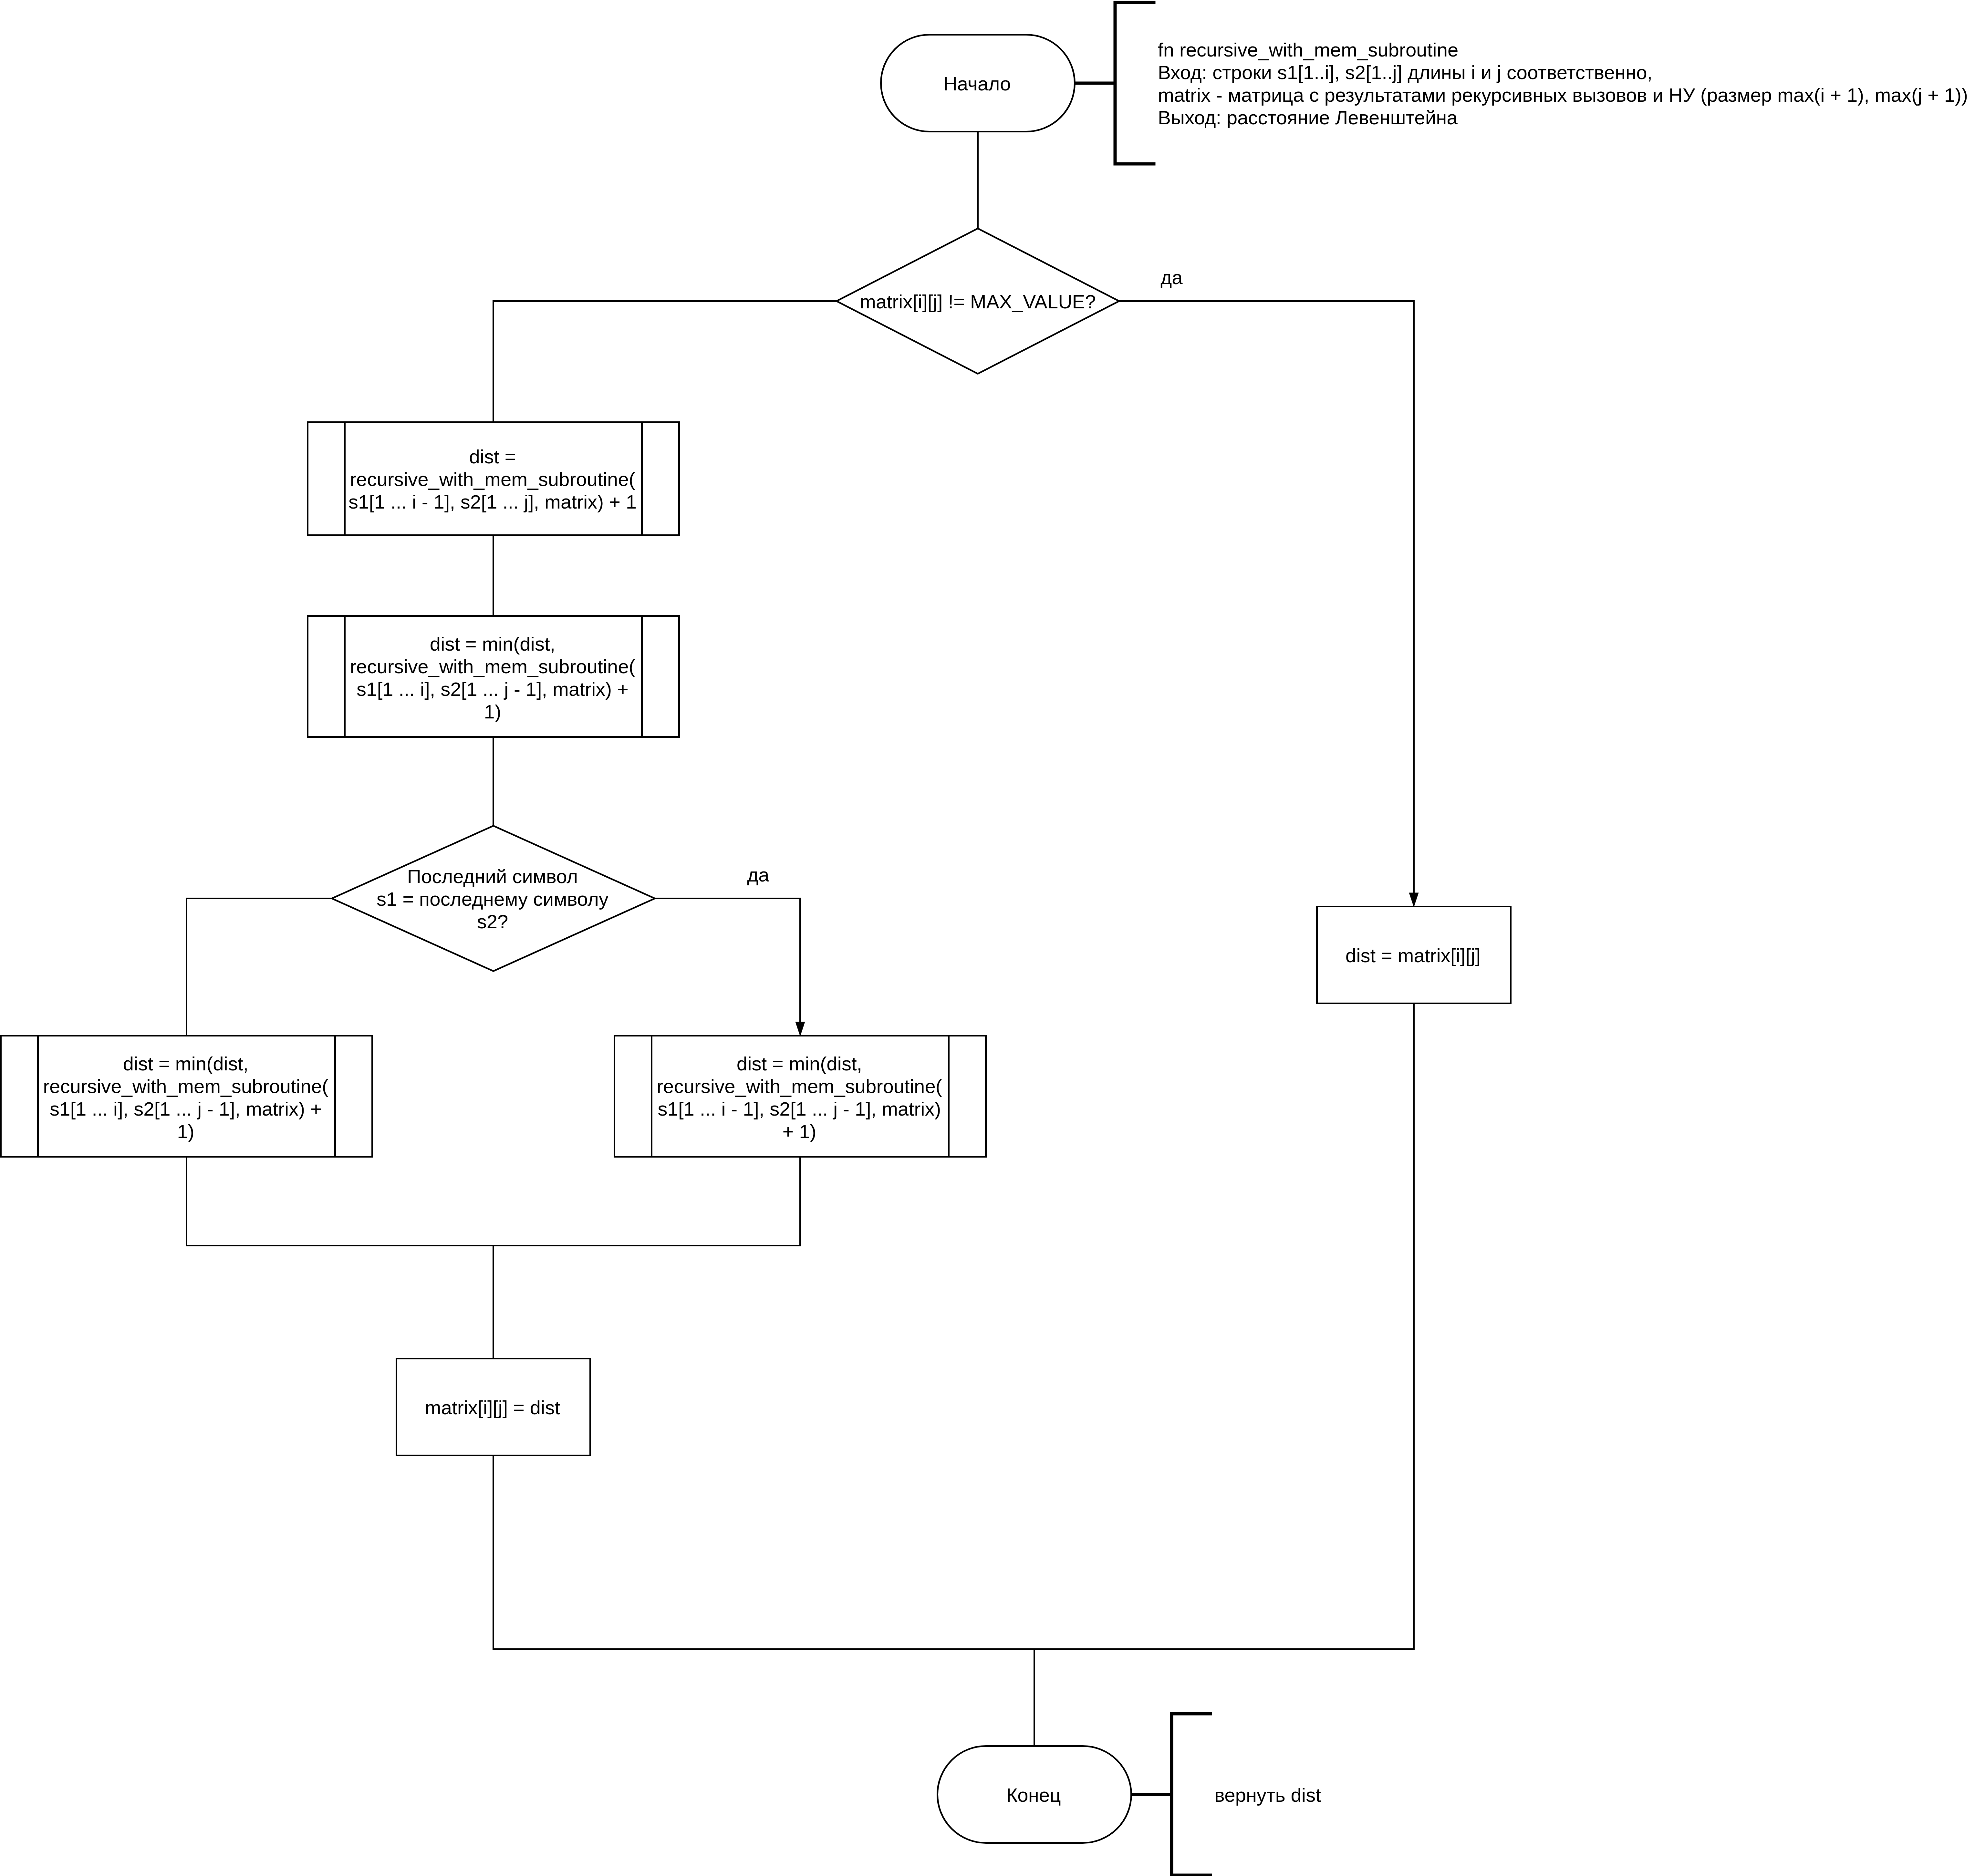
\includegraphics[width=180mm]{inc/img/recursive_with_mem.png}
\caption{Схема процедуры рекурсивного алгоритма нахождения расстояния Дамерау-Левенштейна с заполнением матрицы}
\label{img:recursive_with_mem}
\end{figure}

\img{220mm}{iterative}{Схема матричного алгоритма нахождения расстояния Левенштейна}
\img{220mm}{iterative_dl}{Схема матричного алгоритма нахождения расстояния Дамерау-Левенштейна}
\img{220mm}{iterative_dl_2}{Продолжение схемы матричного алгоритма нахождения расстояния Дамерау-Левенштейна}
